Extracted from ConditionalLoops.tex%\hrule\vskip 1ex
%\begin{minipage}[t]{\linewidth}
%\hfil 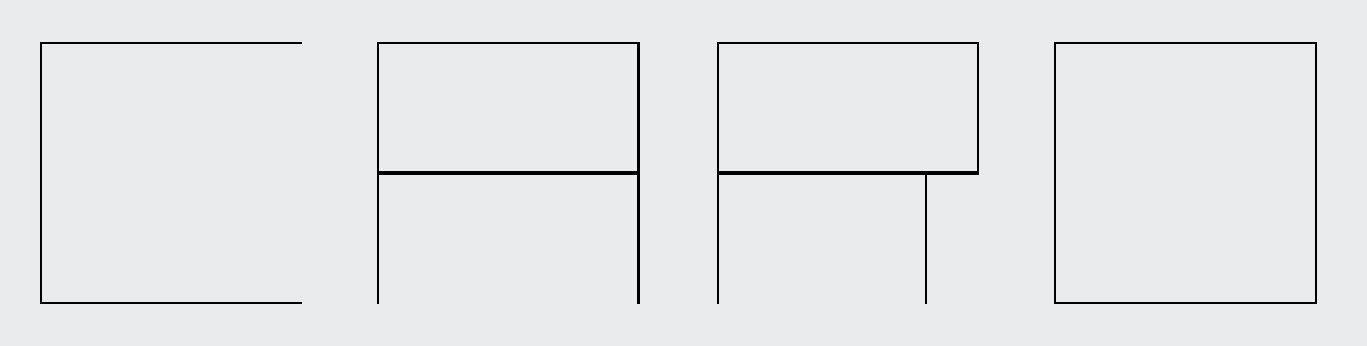
\includegraphics[width=0.9\linewidth]{carosName}\hfil
%\end{minipage}
%\vskip 1ex\hrule\vskip 5ex

\forreviewers{underway}
Up to now the messages sent  to a turtle to change its location were relative to
its current position. Indeed, 
\ct{caro\ go:\ 100} pixels means that we ask a turtle named caro to go forward 100 pixels 
from its current position in its current direction. Such move is said to be
 \emph{relative} because the
position reached by the turtle at the end of the move depends on its
initial position. This kind of move is very powerful but sometimes you would like
to be able to say: \emph{caro go there} where \strong{there} is a
given location on the screen. This means that you would like to
make a turtle move in a \strong{absolute} manner.


In this chapter we will present new turtle behavior that will make the turtle change its location in an absolute manner.
 This will help us to explore new problems in the future such as using turtles to simulate animal behavior. To be able to designate a location on the screen we will introduce the class \ct{Point}\index{Point} which defines the mathematical behavior of point objects.  Points are  important and we will use in the future chapters. 


\begin{figure}
\begin{center}
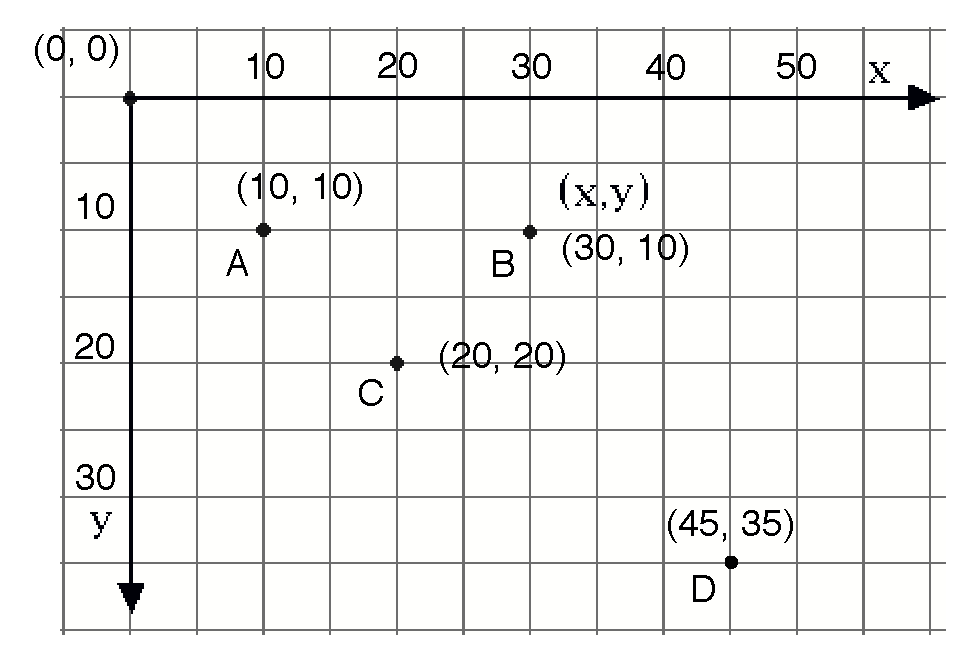
\includegraphics[width=8cm]{PointsReperes}
\caption{Points and Rectangles. \label{fig:PointsRepere}}
\end{center}
\end{figure}

\section{Points}
Since Squeak is an object-oriented language, locations on the screen is {\em also} described 
by objects called \emph{points}. Squeak points are created by the class \ct{Point} and their behavior is close to the mathematical one.  In two dimensions a point is composed by two coordinates: $x$ (the point abscissa) and $y$ (the point ordinates). 
In Smalltalk points are represented and created using the \ct{@}\index{@} method. For example, the point A of Figure~\ref{fig:PointsRepere} is created and represented as \ct{75@50}. A's abscissa is \ct{75} and ordinates is \ct{50}. 
Figure~\ref{fig:PointsRepere} shows that contrary to the mathematical model, the y axis goes positive from the top to the bottom of the screen while the x axis does not change and goes increasing  from left to right. Thus, the point \ct{75@50} is located 75 pixels from the left hand side of the screen and 50 pixels from the bottom of the screen.

\cadre{200@400 is a point whose abscissa is 200 and ordinates 400.}

\begin{figure}
\begin{center}
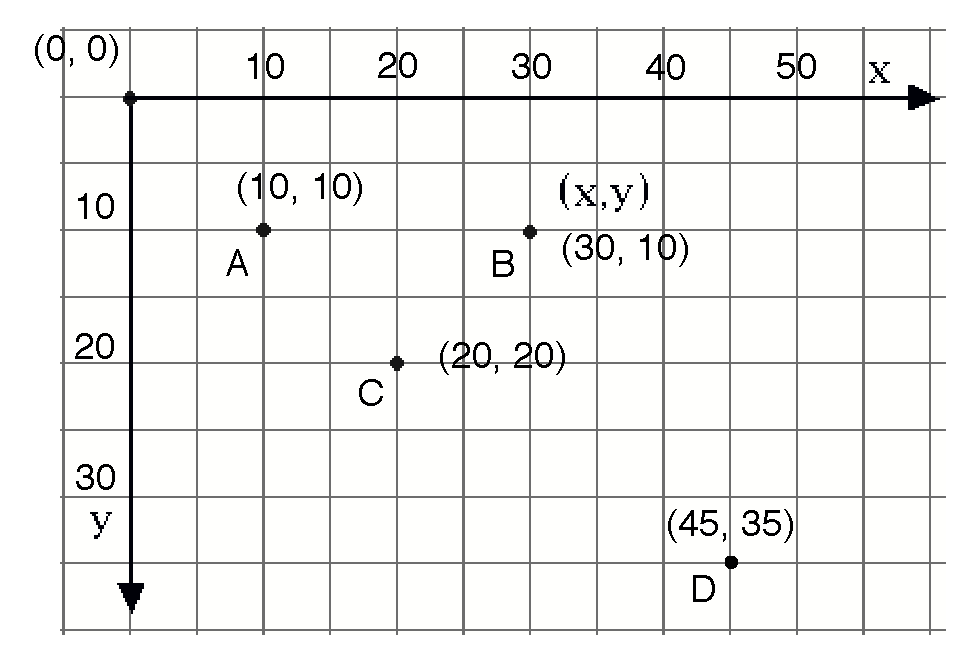
\includegraphics[width=8cm]{PointsReperes}
\caption{Points and Rectangles. \label{fig:PointsRepere}}
\end{center}
\end{figure}

All kinds of mathematical operations are available on the points. We will here only present some of them. If you need information about points use the practices presented in the chapter charef{} to query the system and find the behavior you need.

\paragraph{Point Creation.}
The expression \ct{200@400} creates a point at the location 200 following the axis x and 400 following the axis y. \ct{@}\index{@} sent to a number creates a point whose x is the number and y is the argument passed. The other way of creating a point is to use the following expression \ct{Point x: 200 y: 400} which is equivalent to \ct{200@400} but much longer to type. 


The following script ~\scrref{scr:pointope} presents how to access point constituents. 
\begin{scriptwithtitle}{Point element access}\label{scr:pointope}
| point1 point2 point3 |
point1 := 200@400.
point 1 x
-> 200
point1 y 
-> 400
\end{scriptwithtitle}

Smalltalk goes a step further. We can for example multiply a point by a value to get a point whose values is the previous ones but  multiplied by this value, or use common mathematical operation such as addition, substraction on points themselves. Note that the binary operations such as -, *, + creates new points.  The script~\ref{scr:pointmultiple}  shows how a point gets multiply. 

\begin{scriptwithtitle}{Point manipulation}\label{scr:pointmultiple}
| point1 point2 point3 |
point1 := 200@400.
point2 := point1 * 2
point2 x
-> 400
point2 y
-> 800
point3 := (50@60) + point1.
point3 x
-> 250
point3 y
-> 460
point1 + 200      "200 is considered as the point 200@200"
-> 400@400
\end{scriptwithtitle}

The way points are created may lead to some errors as shown by the first line of the \scrref{scr:pointprob} that returns aB3dVector instead of a point. 

\begin{scriptwithtitle}{Possible error with points}\label{scr:pointprob}
50@60 + 200@400
->  a B3DVector3(250.0 260.0 400.0)
"returns a 3D vector but not a point"

(50@60) + (200@400)
-> 250@460
\end{scriptwithtitle}

\begin{astuce}
To avoid trouble with points, surround them with parenthesis when they are involved in complex operation.
\end{astuce}

\begin{spicy}
As explained in\charef{} and \charef{}, remember that () are evaluated first and there are three weights {\em unary} the heavier, {\em binary}, and {\em keywords} the ligther and that we {\em always start by executing the heavier first} and from left to right when the selectors have the same weight.  In fact the method \ct{@} is just like any other methods and as the same weight that binary methods such as +, *, or //. 

In Smalltalk when we compose messages with selector having the same weight we start form left to right like when writing. 
Hence, the expression \ct{50@60 + 200@400} is equivalent to \ct{(((50@60) + 200) @ 400)}. Let us look at what happens in the first line of the script~\ref{scr:pointprob} which does not correctly returns the point \ct{250@460} as expected. The script~\ref{scr:understanding} shows how the messages are excuted. 
\end{spicy}


\begin{scriptwithtitle}{Decomposing \ct{50@60 + 200@400}}\label{scr:understanding}
50@60 + 200@400 {\rmfamily is equivalent to}(((50@60) + 200) @ 400)
{\rmfamily
{\textbf Step 1}
   \ct{@} is sent to \ct{50} with the argument \ct{60}, it returns the point \ct{50@60}. 
{\textbf Step 2}
   \ct{+} is sent to the point \ct{50@60} with the argument \ct{200}, it returns
   \ct{250@260} because when a number is passed as an argument it is 
   considered as the point having the same value for x and y. 
   Here \ct{200@200}. 
{\textbf Step 3} 
   \ct{@} is sent to \ct{250@260} with \ct{400} as argument, the object
   \ct{B3DVector3(250.0 260.0 400.0)} is returned.}
\end{scriptwithtitle}


\begin{scriptwithtitle}{Decomposing \ct{(50@60) + (200@400)}}\label{scr:understanding2}
(50@60) + (200@400)
{\rmfamily
{\textbf Step 1} 
   Parenthesis are evaluated first.
{\textbf Step 1.1} 
  \ct{@} is sent to \ct{50} with \ct{60} as argument and returns a point.
{\textbf Step 1.2} 
  \ct{@} is sent to \ct{200} with \ct{400} as argument and returns a point.
{\textbf Step 2} 
   \ct{+} is sent to \ct{50@60} with argument \ct{200@400} and 
    returns the new point \ct{250@460}.}
\end{scriptwithtitle}



\section{Absolute Moves}
Now that we can specify location on the screen, we want to ask a turtle to go directly at a given location. For this task we defined two 
methods \lgoat\index{goAt:} and  \ljumpat\index{jumpAt:}.The method \ct{goAt:} asks a turtle to go to a
location specified by the coordinates of a point. While moving the
turtle leaves a trace on the screen. The method \ljumpat asking a turtle to position
itself on the given point without leaving a trace. 

The result of the script~\ref{scr:moveToPoint} shown in Figure~\ref{fig:goatjump} depends on the resolution of your computer. But a turtle draws a line from the current center of the screen to the location 200@400, then it jumps 100 pixels to the right, draws one dot, jumps again 100 pixels to the right and draws a line of 50 pixels. The following section will stress the difference the methods \ct{go: aDistance} and \lgoat, and \ct{jump: aDistance} and \ljumpat.

\begin{scriptwithtitle}{Going directly at a location and jumping.}\label{scr:moveToPoint}
| caro  |
caro := Turtle new.
caro goAt: 200@400.
caro jumpAt: 300@400.
caro go: 1.
caro jumpAt: 400@400.
caro goAt: 450@400
\end{scriptwithtitle}

\begin{figure}
\begin{center}
\includegraphics[width=8cm]{goAtJumpAt}
\caption{\lgoat places a turtle at a given screen location and let a trace from 
its current location to the specified one. \ljumpat places a turtle at a given 
screen location without  letting a trace. \label{fig:goatjump}}
\end{center}
\end{figure}


%\begin{scriptfig}{goAtJumpAt}{Going directly at a location and jumping.}\label{scr:moveToPoint}
%| caro  |
%caro := Turtle new.
%caro goAt: 200@400.
%caro jumpAt: 300@400.
%caro go: 1.
%caro jumpAt: 400@400.
%caro goAt: 450@400
%\end{scriptfig}


\section{Relative vs Absolute Motions}
Let us look at the difference between the methods  \ct{go: aDistance} and \lgoat.
The method \lgo asks a turtle to go for a given distance \emph{along its current direction}. Thus, the position of
the turtle depends on its current location and of its current
direction. The \scrref{scr:moveToPoint} illustrates this.

\begin{scriptfig}{dualMotion}{Parallel motion}
\label{scr:dualMotion}
| caro marge |
caro := Turtle new.
marge := Turtle new.
marge north.
marge jump: 100.
marge east.
caro go: 300.
marge go: 300.
\end{scriptfig}

As you can see, the two turtles are moving along parallel lines and
do not end up in the same location, even though the same message
\ct{go:\ 300} was issued to them at the end of the script.

On the contrary, the method \lgoat asks a turtle to place itself
to a fixed location regardless of its position and direction
before the move. This is illustrated by
\scrref{scr:convergentMotion}.

\begin{scriptfig}{convergentMotion}{Convergent motion}
\label{scr:convergentMotion}
| caro marge |
caro := Turtle new.
marge := Turtle new.
marge lookLikeTriangle.
marge penSize: 3.
marge north.
marge jump: 100.
marge east.
caro goAt: 300@200.
marge goAt: 300@200.
marge go: 100 
\end{scriptfig}

In this case, the two turtles end up at the same location. One
says that the method \go produces a \emph{relative}
motion, whereas the method \goat produces an
\emph{absolute} motion.

Finally it should be noted that the methods \go and \goat do not
change the direction of the turtle. This is illustrated by
\scrref{scr:combinedMove}. In this script we ask a turtle to move forward 100 pixels from its current position, then 
asks it to go directly to a position that is located at 100, -100 from the center of the screen, and then move forward again 100.

\begin{scriptfig}{combinedMove}{Combining absolute and relative motions}
\label{scr:combinedMove}
| caro |
caro := Turtle new.
caro north.
caro go: 100.
caro goAt: (World center - (100@-100)).
caro go: 100.
\end{scriptfig}



\begin{spicy}
Smalltalk is a uniform language in which {\em everything} is an object to which we sent messages. This applies to points as well. 
 In fact the expression \ct{200@600} that creates a point is a message sent to an
object, an integer.  Here the method \ct{@} is sent to 200 with argument the integer 600. \ct{@} is defined on the class \ct{Integer}
and returns a new point having the receiver as x and the argument as y.
\end{spicy}


\section{Experiments}
Before going any further we propose you some experiences you get more familiar with the concepts presented. Note that 
using the animated turtle can really help you here. 

\begin{exonofig}
Experiment to guess the size of your screen in pixels.
\end{exonofig}

\begin{exofig}{rectangle} \label{exo:rectangle}
Using the methods \goat and \jumpat draw a rectangle using two points that represent its opposite corners. 
For example, use 200@600 and 350@500.
Hint: First, draw on paper the points, then decompose the steps that the turtle should follow. 
\end{exofig}

\comment{
\begin{scriptwithtitle}{Absolute Rectangle}| caro point1 point2|
caro := AniTurtle new.
point1 := 350@500.
point2 := 200@600.
caro jumpAt: point1.
caro goAt: point1 x @ point2 y.
caro goAt: point2.
caro goAt: point2 x @ point1 y.
caro goAt: point1
\end{scriptwithtitle}
}

\begin{exonofig}\label{exo:rectangle2}
Transform the \scrref{exo:rectangle} so that the second point does not represent anymore the opposite corner but the size of the rectangle. For example we will have a rectangle starting at location 200@600 and having a height of 350 and width of 500. \end{exonofig}

\begin{exonofig}
Transform the script \scrref{exo:rectangle} into the methods \ct{rectangleOrigin: aPoint1 corner: aPoint2}. \ct{aTurtle rectangleOrigin: 200@600 corner: 350@500}.
Transform the \scrref{exo:rectangle2} into the method \ct{rectangleOrigin: aPoint1 extent: aPoint2}. \ct{aTurtle rectangleOrigin: 200@600 extent: 350@500}
\end{exonofig}


\section{Translations}
In mathematics, a translation is defined as the operation of
moving a geometrical shape without modifying its shape. Points can
be used effectively to represent a translation: a translation
consists of adding two constants to all points defining the shape.
Since this operation is quite important, Smalltalk defines the
addition between points as a new point having for abscissa the sum
of the abscissa and for ordinate the sum of the ordinates of the
two points. The script \scrref{scr:pointmultiple} presents such behavior.

The script~\scrref{scr:combinedMove} draws a triangle in absolute coordinates 
before and after a translation of \ct{50@75}.

\begin{scriptfig}{translation}{Translation of a triangle}\label{scr:combinedMove}
| caro point1 point2 point3 translation |
point1 := 200@300.
point2 := 200@250.
point3 := 150@300.
translation := 50@75.
caro := Turtle new.
caro jumpAt: point1.
caro goAt: point2.
caro goAt: point3.
caro goAt: point1.
point1 := point1 + translation.
point2 := point2 + translation.
point3 := point3 + translation.
caro jumpAt: point1.
caro goAt: point2.
caro goAt: point3.
caro goAt: point1.
\end{scriptfig}

One can repeat the translation operation to obtain repeating
patterns. The script~\scrref{scr:flyingGeese} generates the pattern called \emph{flying
geese} in patchwork. Here we modify the amount of translation so that the next triangle is 
in diagonal.

\begin{scriptfig}{flyingGeese}{Flying geese}\label{scr:flyingGeese}
| caro point1 point2 point3 translation |
point1 := 200@300.
point2 := 200@250.
point3 := 150@300.
translation := 25@25.
caro := Turtle new.
10 timesRepeat: [
       caro jumpAt: point1.
       caro goAt: point2.
       caro goAt: point3.
       caro goAt: point1.
       point1 := point1 + translation.
       point2 := point2 + translation.
       point3 := point3 + translation].
\end{scriptfig}

\subsection{Improving the Design of Flying Geese}
The scripts~\scrref{scr:combinedMove} and \ref{scr:flyingGeese} are not really well defined because
the is a lot of behavior that is duplicated and we cannot reuse the elementary operations that are used such a drawing a triangle and translating to a new position. Again this is an example showing the power of decomposing complex problems into smaller ones.  To fix that situation we need to define one method for drawing a triangle and one for translating the receiver. 

\paragraph{Triangle.}
Define a method named \ct{triangleAt: point1 point2: point2 point3: point3} which draws a triangle
 between the points given as arguments. \Tscrref{scr:triangle} illustrates how to use such a method and Figure~\ref{fig:triangleByPoints} shows its result.


\begin{scriptfig}{triangleByPoints}{Using \ct{triangleAt:point2:point3:}}\label{scr:triangleUse}
| caro |
caro := Turtle new.
caro  
   triangleAt: 200@300 
   point2: 200@250 
   point3: 150@300 
\end{scriptfig}

\begin{exofig}{triangleByDelta}
Define another method named \ct{triangleAt: aPoint delta1: aPoint1 delta2: aPoint2} that starts to draw a triangle at aPoint then uses the two following arguments as differences by reference to the original point and the second point.
So that \ct{t triangleAt: 200@300 delta1: 0@-50 delta2: -50@50} draws the same triangle as: 
\ct{t triangleAt: 200@300 point2: 200@250 point3: 150@300}
\end{exofig}


\paragraph{Re-expressing \tscrref{scr:flyingGeese}.}
Using the new method we defined the script looks simpler. 

\begin{scriptwithtitle}{New Version of Flying Geese}\label{scr:newflyinggeese}
| caro translation point1 point2 point3 |
point1 := 200@300.
point2 := 200@250.
point3 := 150@300.
translation := 25@25.
caro := Turtle new.
10 timesRepeat: [
	caro triangleAt: point1 point2: point2 point3: point3.
       point1 := point1 + translation.
       point2 := point2 + translation.
       point3 := point3 + translation].
\end{scriptwithtitle}



\section{Using points}
Why does one need points? So far, all drawings did not require points. 
For that matter executing most drawings using points
would have been quite difficult. Imagine how difficult can be  to draw a pentagon. 
Still absolute positions are useful. The following illustrates such an example. 

We will use a point to recover the position of a turtle at a given time during the 
execution of a complex drawing. The first example refers to the \scrref{scr:letterA} of
chapter \ref{ch:turtleMen}. At the end of Section \ref{sec:abcDraw} we noted that the bottom
half of the left bar of the "A" is drawn twice by the 
\scrref{scr:letterA}. We considered that it was not
that big a problem since we considered that \emph{computer
paint} is not expensive. Nevertheless, for some drawing, going
over previously drawn lines could be \emph{computer expensive}. By
\emph{computer expensive} we mean that reproducing previously
drawn lines requires complex computation and/or needs a large
number of methods. In this case, drawing lines twice becomes
indeed a problem.

The solution is to use a point to store the location of the
turtle, location to which the drawing requires to come back later.
Let us modify the \scrref{scr:letterA} as follows to illustrate
this technique. At the same time, the new script is using relative
orientation so that it can draw the letter "A" at any orientation.

\begin{scriptfig}{letterAWithPoint}{The letter "A" is any direction}\label{scr:absoluteA}
|caro barPoint|
caro := Turtle new.
caro beInvisible.
caro turnLeft: 90.
caro go: 40.
{\textbf barPoint := caro center}.
caro go: 60.
caro turnRight: 90.
caro go: 70.
caro turnRight: 90.
caro go: 100.
{\textbf caro jumpAt: barPoint.}
caro turnLeft: 90.
caro go: 70.\end{scriptfig}

In \scrref{scr:absoluteA}, the first vertical bar of the "A"
is drawn in two steps. Between the steps, the absolute location of
the turtle is obtained using the method \ct{center}\index{center}.
This is the location where the bar of the "A" should be drawn. The
result of that method is stored in the variable
\ct{barPoint}. After the last vertical bar is drawn, the turtle goes back to the
location of the bar using the method \ct{goAt:\
barPoint}. From this point on, the bar is drawn.

\begin{figure}
\begin{center}
\includegraphics[width=8cm]{centerPosition}
\caption{The difference between \ct{center} and \ct{position}. \label{fig:centerPosition}}
\end{center}
\end{figure}

You can verify that the letter "A" is indeed drawn correctly in
any direction by adding a command \ct{turnLeft:} or
\ct{turnRight:} after the creation of the turtle. 



\begin{exofig}{arrows} \label{exo:arrows}
Using the same technique, define a script that generates 8 arrows shooting from the turtle
origin in 8 different directions as shown in the neighboring
figure. The script must use the command \ct{timesRepeat:}.
Hint: Define first a method called \ct{arrow: aPoint} that draws an arrow pointing in the current 
direction starting at the given point. Then use a additional variable to remember the origin of the arrow.
\end{exofig}

\section{Loops and translations}
Now we explain how we can produce the drawing shown in Figure~\ref{scr:flyingGeeseQuit}. 
Points definea lot of useful method from which we explain first the ones we used to the full quilt cover
with flying geese shown in Figure~\ref{scr:flyingGeeseQuit}.

The method \ct{negated} sent to a point returns a point whose
abscissa and ordinate are negated value of the receiving
point. Thus, the point \ct{(200@400)\
negated} is the point \ct{-200@-400}. Note that the
parentheses are necessary. Indeed, \ct{negated} is also a
method understood by numbers. Thus, the expression
\ct{200@400\ negated} yields the point \ct{200@-400}
because the method \ct{negated} being an unary method 
is executed before the method \ct{@} by the
number \ct{400}. In \tscrref{scr:flyingGeeseQuit} we use this
method to produce a translation in the opposite direction.

The method \ct{setX:setY:} changes the constituents of a point.
Thus, if \ct{point} is any point, after executing the expression
\ct{point\ setX: 200\ setY: 400}, the point has for x value \ct{200} and for y value \ct{400}. 


\Tscrref{scr:flyingGeeseQuit} uses these two methods within a double loops
to generate the flying geese pattern over a large region
of the screen. The inside loop is following the spirit of the 
\tscrref{scr:newflyinggeese} except that the orientation of the triangle
and that of the translation are rotated so that a line of
triangle is now horizontal. The outside loop makes a translation
of the last triangle to bring it atop the line of triangle using
the point variable \ct{shift}; then, the translation are reversed so
that the next line is drawn in reverse order. The triangles,
however, are still drawn with the same orientation. The fact that
a second line of triangles appears to point in the opposite
direction results from the fact that the two lines of triangles
touch themselves. Note that the variable \ct{shift} must be
transformed in a special way: the sign of its abscissa is reversed
at the end of each line to compensate for the last translation
which is not drawn.

\begin{scriptfig}{flyingGeeseQuit}{Flying geese cover quilt}
\label{scr:flyingGeeseQuit}
| caro point1 move shift|
point1 := 200@300.
move := 25@0.
shift := -25@50.
caro := Turtle new.
5 timesRepeat: [
   10 timesRepeat: [
       caro 
          triangleAt: point1 
          delta1: 25@-25 
          delta2: -25@-25.
       point1 := point1 + move].
   point1 := point1 + shift.
   move := move negated.
   shift setX: shift x negated setY: shift y].
\end{scriptfig}

\section{Further Experiments}
\paragraph{The method \ct{translate: aPoint}.}
Defining methods with a precise and simple behavior is a way to simplify your code
as explained in~\charef{ch:recomposing}. Define the method \ct{translate: aPoint}\index{translate:}. Before looking at the solution we propose in \mthref{mth:translate}, propose an implementation. 

\begin{method}\label{mth:translate}
translate: aPoint
   "translate the receiver of aPoint x and aPoint y"
		
   self goAt: (self center + aPoint)	
\end{method}

Propose a different method \ct{translateX: x y: y} which takes as argument the value for x and y separately. 

\begin{exonofig}
Change the definition of  the method \ct{triangleAt:point2:point3:} to use the method \ct{translate: aPoint}.
\end{exonofig}


\subsection{Commands summary}
Here is the list of the commands, which you have learned in this
chapter.
\begin{table}[h]
  \centering
  \caption{Commands introduced in Chapter \ref{ch:absoluteLocation}}\label{tbsum:absoluteLocation}
\begin{tabular}{| l | p{5cm} | l |} \hline
  % after \\ : \hline or \cline{col1-col2} \cline{col3-col4} ...
  \hfil Command & \hfil Description & \hfil Example \\[1ex] \hline
  $x$\ct{\ @\ }$y$ & Creates a point of given coordinates &
  \ct{300\ @\ 600} \\
  \ct{goAt: aPoint} & Ask a turtle to move to a given point & \ct{caro\ goAt:\ 300\ @\ 600} \\
  \ct{jumpAt: aPoint} & Position a turtle to a given point & \ct{caro\ jumpAt:\ 300\ @\ 600} \\
  \ct{point1 + point2} & Construct a point whose components are the sum of the components of two given points & \ct{50\ @\ 200\ +\ 300\ @\ 600} \\
  \ct{point1 negated} & Construct a point whose components are the opposite of the original point & \ct{(50\ @\ 200)\ negated} \\
  \ct{center} & Returns the current position of a turtle as a point & \ct{barPoint\ :=\ caro\ center} \\
  \hline
\end{tabular}
\end{table}



\ifx\wholebook\relax\else\end{document}\fi
